\chapter{Theoretical Framework}\label{chap:theory}

\begin{itemize}
  \item Introduce sm
  \item brief history
  \item current areas of study
  \item Reference relevenace to rest of thesis (studying hbb)
\end{itemize}

The Standard Model (SM) of particle physics is the theory describing all known elementary particles and their interactions via three of the four fundamental forces.
Developed by merging the successful theories of classical quantum mechanics and relativity in the second half of the 20th century, the SM's position today at the centre of our understanding of the nature of the universe is firmly established by an unparalleled level of agreement between the predictions from the model and experimental results \cite{morel2020determination,sailer2022measurement}.

The SM has predicted the discovery of the top and bottom quarks \cite{CDF:1995wbb,D0:1995jca,Herb:1977ek}, the \Wboson and \Zboson bosons \cite{UA1:1983crd}, and the tau neutrino \cite{DONUT:2000fbd}.
The last missing piece of the SM to be discovered was the Higgs boson, first posited in \tofill{X}.
After its discovery in 2012 \tofill{citation}, much work has been ongoing on carrying out detailed measurements of its mass and interactions with other particles.

This thesis looks at understanding Higgs decays\dots


\section{The Standard Model}\label{sec:standard_model}

The SM is formulated in the language of Quantum Field Theory (QFT).
In this framework, particles are localised excitations of corresponding quantum fields, which are operator-valued distribution across spacetime.

Central to QFT is the Lagrangian density which describes the kinematics and dynamics of a field.
Observations of conserved quantities are linked, via Noether's theorem, to symmetries which are expressed by the Lagrangian.
Alongside Global Poincar\'e symmetry, the SM Lagrangian observes a local non-Abelian $SU(3)_C \otimes SU(2)_L \otimes U(1)_Y$ gauge symmetry.
Gauge symmetries leave observable properties of the system unchanged when certain gauge transformations are applied to the fields.
The full Lagrangain of the SM can be broken up into distinct terms corresponding to the different sectors.
%
\begin{equation}\label{eq:sm_lagrangian}
  \mathcal{L}_{\textnormal{SM}} = \mathcal{L}_{\textnormal{EW}} + \mathcal{L}_{\textnormal{QCD}} + \mathcal{L}_{\textnormal{Higgs}} + \mathcal{L}_{\textnormal{Yukawa}}
\end{equation}
%
The SM provides a mathematical description of how the four fundamental forces interact with the matter content of the universe.
The SM contains $12$ \spinhalf fermions, listed in \cref{tab:sm_fermions}, and $5$ bosons listed in \cref{tab:sm_bosons}.
%
\begin{table}[!htbp]
  \footnotesize\centering
  \setlength{\tabcolsep}{0.5em} % for the horizontal padding
  \begin{tabular}{c|ccc|ccc}
      \toprule 
      \multicolumn{1}{c|}{} & \multicolumn{3}{c|}{Leptons} & \multicolumn{3}{c}{Quarks} \\
      \hline
      \textbf{Generation} & \textbf{Flavour} & \textbf{Mass} [\unit\MeV] & \textbf{Charge} [\unit\elementarycharge] & 
                            \textbf{Flavour} & \textbf{Mass} [\unit\MeV] & \textbf{Charge} [\unit\elementarycharge] \\
      \hline
      \multirow{2}{*}{First} & 
        $e$        & $0.511$               & -1 & $u$ & $2.16$ & \nicefrac{2}{3} \\
      & $\nu_e$    & $<1.1 \times 10^{-6}$ &  0 & $d$ & $4.67$ & \nicefrac{-1}{3} \\
      %
      \hline
      \multirow{2}{*}{Second} & 
        $\mu$      & $105.7$ & -1 & $c$ & $1.27 \times 10^{3}$ & \nicefrac{2}{3} \\
      & $\nu_\mu$  & $<0.19$ &  0 & $s$ & $93.4$               & \nicefrac{-1}{3} \\
      %
      \hline
      \multirow{2}{*}{Third} & 
        $\tau$     & $1776.9$& -1 & $t$ & $173 \times 10^{3} $ & \nicefrac{2}{3} \\
      & $\nu_\tau$ & $<18.2$ &  0 & $b$ & $4.18  \times 10^{3} $ & \nicefrac{-1}{3} \\
      \bottomrule
  \end{tabular}
  \caption{
    The half-integer spin fermions of the SM \cite{Workman:2022ynf}.
    Three generations of particles are present.
    Also present (unlisted) are the antiparticles, which are identical to the particles up to a reversed charge sign.
    }
  \label{tab:sm_fermions}
\end{table}
%

%
\begin{table}[!htbp]
  \footnotesize\centering
  \setlength{\tabcolsep}{0.5em} % for the horizontal padding
  \begin{tabular}{lcccc}
      \toprule 
      \textbf{Name} & \textbf{Symbol} & \textbf{Mass} [\unit\GeV] & \textbf{Charge} [\unit\elementarycharge] & \textbf{Spin} \\
      \hline
      Photon      & \photon   & $< 1 \times 10^{-27}$     & $< 1 \times 10^{-46}$      & 1    \\
      Weak boson  & \Wpm      & $80.377 \pm 0.012$     & $\pm 1$    & 1    \\
      Weak boson  & \Zboson   & $91.1876 \pm 0.0021$     & 0    & 1    \\
      Gluon       & \gluon    & 0     & 0.5    & 1    \\
      Higgs       & \higgs    & $125.25 \pm  0.17$     & 0    & 0    \\
      \bottomrule
  \end{tabular}
  \caption{
    The integer spin bosons of the SM \cite{Workman:2022ynf}.
    The photon, weak bosons and gluons are gauge bosons arising from gauge symmetries, and carry the four fundamental forces of the SM.
  }
  \label{tab:sm_bosons}
\end{table}
%
\begin{comment}
  In quantum physics and chemistry, quantum numbers describe values of conserved quantities in the dynamics of a quantum system. Quantum numbers correspond to eigenvalues of operators that commute with the Hamiltonian—quantities that can be known with precision at the same time as the system's energy[note 1]—and their corresponding eigenspaces. Together, a specification of all of the quantum numbers of a quantum system fully characterize a basis state of the system, and can in principle be measured together.
\end{comment}


\subsection{Quantum Electrodynamics}\label{sec:qed}

Consider a Dirac spinor field $\psi = \psi(x)$ and its adjoint $\overline{\psi} = \psi^\dagger \gamma^0$, where $\psi^\dagger$ denotes the Hermitian conjugate of $\psi$.
The field $\psi$ describes fermionic \spinhalf particle, for example an electron.
The Dirac Lagrangian density is
%
\begin{equation}\label{eq:dirac_lagrangian}
  \mathcal{L}_{\textnormal{Dirac}} = \overline{\psi} (i \slashed{\partial}  - m )\psi,
\end{equation}
%
where $\slashed{\partial} = \gamma^\mu \partial_\mu$ denotes the contraction with the Dirac gamma matrices $\gamma^\mu$ (summation over up-down pairs of indices is assumed).
Application of the Euler-Lagrange equation on \cref{eq:dirac_lagrangian} yields the Dirac equation\todo{mention EoMs?}
%
\begin{equation}\label{eq:dirac_eq}
  (i \slashed{\partial}  - m )\psi = 0 .
\end{equation}
%
Suppose some fundamental symmetry that requires invariance under a $U(1)$ local gauge transformation
%
\begin{equation}\label{eq:U(1)_transformation}
  \psi \rightarrow \psi' = \psi e^{- i q \alpha(x)} ,
\end{equation}
%
where $\alpha$ varies over every spacetime point $x$.
Under this transformation, the Dirac equation transforms as 
%
\begin{equation}\label{eq:dirac_eq_transformed}
  (i \slashed{\partial} - m ) \psi e^{- i q \alpha(x)} + q \slashed{\partial}\alpha(x) \psi e^{- i q \alpha(x)} = 0.
\end{equation}
%
For the Dirac equation to remain invariant under the transformation in \cref{eq:U(1)_transformation}, a new field $A_\mu$ which transforms as $A_\mu \rightarrow A'_\mu = A_\mu + \partial_\mu \alpha(x)$ must be added.
The transformed interaction term
%
\begin{equation}
  - q \slashed{A} \psi \rightarrow - q \slashed{A} \psi e^{- i q \alpha(x)} - q \slashed{\partial} \alpha(x) \psi e^{- i q \alpha(x)}
\end{equation}
%
will then cancel the asymmetric term in \cref{eq:dirac_eq_transformed} as required.
The $U(1)$ invariant Lagrangain can therefore be constructed by adding an interaction between $\psi$ and $A_\mu$ to \cref{eq:dirac_lagrangian}. The kinetic term for the the new field $A_\mu$ is also added in terms of $F_{\mu\nu} = \partial_\mu A_\nu - \partial_\nu A_\mu$, which is trivially invariant under the transformation in \cref{eq:U(1)_transformation}.
The interaction term is absorbed into the covariant derivative $D_\mu = \partial_\mu + i q A_\mu$, thus named as it transforms in the same way as the field $\psi$.
This yields the QED Lagrangain
%
\begin{equation}\label{eq:qed_lagrangian}
  \mathcal{L}_{\textnormal{QED}} = -\frac{1}{4} F_{\mu\nu} F^{\mu\nu} + \overline{\psi} (i \slashed{D} - m )\psi ,
\end{equation}
%
A quadratic term $A_\mu A^\mu$ is not invariant and therefore the the field $A_\mu$ must be massless.
Requiring invariance under local $U(1)$ gauge transformations necessitated the addition of a new field $A_\mu$, corresponding to photons, which interact with charged matter. \todo{improve interpretation}


\subsection{Quantum Chromodynamics}\label{sec:qcd}

Quantum Chromodynamics (QCD) is the study of quarks, gluons and their interactions.
Quarks and gluons carry colour charge, which comes in three kinds, called red, green and blue.
While the $U(1)$ symmetry group in \cref{sec:qed} was Abelian, the QCD Lagrangian is specified by requiring invariance under transformations from the non-Abelian $SU(3)$ group, making it a Yang\nobreakdash-Mills theory \cite{PhysRev.96.191} which requires the addition of self-interacting gauge fields.
The infinitesimal $SU(3)$ group generators are given by $T_a = \lambda_a / 2$, where $\lambda_a$ are the eight Gell\nobreakdash-Mann matrices.
These span the space of infinitesimal group transformations and do not commute with each other, instead satisfying the commutation relation
%
\begin{equation}
  \com{T_a}{T_b} = i f_{abc} T_c ,
\end{equation}
%
where $f_{abc}$ are the group's structure constants.
Consider the six quark fields $q_k = q_k(x)$.
Each flavour of quark $q_k$ transforms in the fundamental triplet representation, where each component of the triplet corresponds to a different value of the colour quantum number.
$G^{a}_{\mu\nu}$ are the eight gluon field strength tensors, one for each generator $T_a$, defined as
%
\begin{equation}\label{eq:qcd_field_strength_tensor}
  G^a_{\mu\nu} = \partial_\mu A_\nu - \partial_\nu A_\mu - g_s f^{abc} A_\mu^b A_\nu^c ,
\end{equation}
%
where $A_\mu^a$ are the gluon fields and $g_s$ is the strong coupling constant. The covariant derivative is written as
%
\begin{equation}\label{eq:qcd_covariant_derivative}
  D_\mu = \partial_\mu + i g_s T_a A_\mu^a .
\end{equation}
%
The full QCD Lagrangain is then given by
%
\begin{equation}\label{eq:qcd_lagrangian}
  \mathcal{L}_\textnormal{QCD} = 
  - \frac{1}{4} G^{a}_{\mu\nu} G_{a}^{\mu\nu}
  + q_k (i \slashed{D} - m_k) q_k .
\end{equation}
%
Cubic and quartic terms of the gauge fields $A^a_\mu$ appear in the Lagrangian, leading to the gluon's self interaction.

The QCD coupling constant $g_s$ varies, or ``runs'', with energy.
At lower energy scales (and corresponding larger distance scales) the interaction is strong.
This leads to quark confinement, whereby an attempt to isolate individual colour-charged quarks requires so much energy that additional quark-antiquark are produced.
At higher energy scales (and corresponding smaller distance scales), asymptotic freedom occurs as the interactions become weaker, allowing perturbative calculations to be performned.
Hadrons are bound states of quarks.
They are invariant under $SU(3)$ gauge transformations (i.e. are colour-charge neutral, or colourless).


\subsection{The Electroweak Sector}\label{sec:ew_sector}

The weak and electromagnetic forces are unified in the Glashow-Weinberg-Salam (GWS) model of electroweak interaction \cite{Glashow:1961tr,Weinberg:1967tq,Salam:1968rm}.
The Lagrangain is specified by requiring invariance under the symmetry group $SU(2)_L \otimes U(1)_Y$, as motivated by a large amount of experimental data.
Here, $SU(2)_L$ is referred to as weak isospin and $U(1)_Y$ as weak hypercharge. (the product of the isospin and hypercharge groups.).

The generators of $SU(2)_L$ are $T_a = \sigma_a/2$, where $\sigma_a$ are the three Pauli spin matrices which satisfy the commutation relation 
%
\begin{equation}
\com{T_a}{T_b} = i \varepsilon_{abc} T_c .
\end{equation}
%
The generator of $U(1)_Y$ is $Y = 1/2$.
Each generator corresponds to an gauge field, which, after symmetry breaking (discussed in \cref{sec:ew_symmetry_breaking}), give rise to the massive vector bosons, \Wpm and \Zboson, and the massless photon.
The massive vector bosons are the carriers of the weak force.

The weak force violates parity conservation \cite{PhysRev.104.254,PhysRev.105.1413,PhysRev.105.1415}, i.e. invariance under parity transformations (mirror reflections).
Only left handed fermions participate in the weak interaction.
There are no right handed neutrinos in the standard model.
The Standard Model incorporates parity violation by expressing the weak interaction as a chiral gauge interaction. Only the left-handed components of particles and right-handed components of antiparticles participate in weak interactions in the Standard Model. The weak force couples only to left handed particles in currents of the form $J^\mu = \overline{\nu}_e \gamma^\mu (1 - \gamma^5) e$ or $J^\mu = \overline{u} \gamma^\mu (1 - \gamma^5) \tilde{d}$. The $\tilde{d}$ state is due to the quark mixing: mass eigenstates are not the same as weak eigenstates.

Furthermore, CP violation has been observed from the weak sector.
CP violation is one of the three necessary Sakharov conditions required to produce baryon asymmetry in the universe.
Since the SM alone does not appear to have enough CP violation to generate the cosmologically observed matter-antimatter asymmetry, looking for signs of more experimental CP violation is considered to be a promising
way to discover new physics.


\section{The Higgs Mechanism}\label{sec:sm_higgs}

Experimentally it was known that the weak forces contains a charged current and had a weak effective strength, suggestive of a massive mediating gauge particle.
However, directly adding mass to the gauge bosons in a non-Abelian theory breaks the symmetry.
Instead, the gauge bosons can gain mass through interaction with a scalar Higgs field, known as the Brout–Englert–Higgs mechanism \cite{Englert:1964et,Higgs:1964pj,Guralnik:1964eu}.
An overview is given below.
%
\begin{figure}[!htbp]
  \centering
  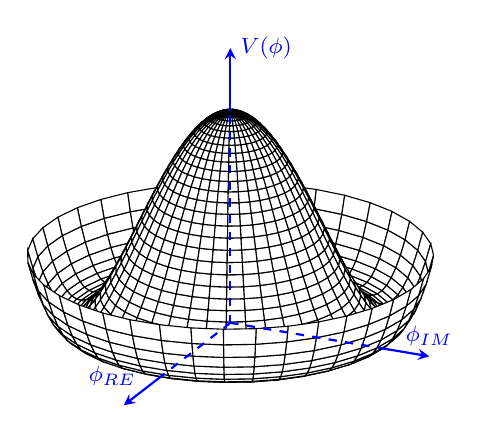
\begin{tikzpicture}

    \begin{axis}[
        %axis lines=center,
        %axis line style={->},
        hide axis,
        samples=40,
        domain=0:360,
        y domain=0:1.25,
        xtick=\empty,
        ytick=\empty,
        ztick=\empty
    ]
    \addplot3 [surf, shader=flat, draw=black, fill=white, z buffer=sort] ({sin(x)*y}, {cos(x)*y}, {(y^2-1)^2});

    \draw[blue,thick,dashed] (axis cs:0,0,0) -- (axis cs:1,0,0)
                %node[below,font=\footnotesize]{$\phi_{\text{IM}}$}
                ;
    \draw[blue,thick,-stealth] (axis cs:1,0,0) -- (axis cs:1.35,0,0)
                node[above,font=\footnotesize]{$\phi_{\text{IM}}$};

    \draw[blue,thick,dashed] (axis cs:0,0,0) -- (axis cs:0,-1,0)
                node[left=2mm,font=\footnotesize]{$\phi_{\text{RE}}$};
    \draw[blue,thick,-stealth] (axis cs:0,-1,0) -- (axis cs:0,-1.55,0)
                %node[right=1mm,font=\footnotesize]{$\phi_{\text{RE}}$}
                ;

    \draw[blue,thick,dashed] (axis cs:0,0,0) -- (axis cs:0,0,1)
                %node[left=2mm,font=\footnotesize]{$\phi_{\text{RE}}$}
                ;
    \draw[blue,thick,-stealth] (axis cs:0,0,1) -- (axis cs:0,0,1.3)
                node[right,font=\footnotesize]{$V(\phi)$};

    \end{axis}

\end{tikzpicture}
  \caption{
    The Higgs potential $V(\phi)$ of the complex scalar field $\phi$, with a choice of $\mu^2 < 0$ leading to a continuous degeneracy in the vacuum states.
  }
  \label{fig:higgs_potential}
\end{figure}
%
Spontaneous symmetry breaking (SSB) is the transition of a physical system from a state of manifest symmetry to a state of hidden, or ``broken'', symmetry. In particular, this applies to physical systems where the Lagrangian observes some symmetry, but the lowest energy vacuum states do not exhibit that same symmetry. The symmetry is broken for perturbations around the vacuum state.

Consider an $SU(2)$ gauge field \todo{cite weak gauge fields, non-Abelian local} coupled with a complex scalar field $\phi$, which transforms as an $SU(2)$ spinor (a weak isospin doublet).
Omitting the kinetic term of the gauge fields, and writing $\phi^2 \equiv \phi^\dagger \phi$, the Lagrangain is
%
\begin{equation}\label{eq:sm_higgs_lagrangian}
  \mathcal{L} = (D_\mu \phi)^\dagger (D^\mu \phi) - \left[ \mu^2 \phi^2 + \lambda \phi^4 \right],
\end{equation}
%
where the covariant derivative is given by
%
\begin{equation}\label{eq:sm_higgs_cov_derivative}
  D_\mu = \partial_\mu + i g A^a_\mu T^a ,
\end{equation}
%
and $T^a$ are the generators of $SU(2)$.
The potential term $V(\phi)$ is made up of a quadratic and quartic term in the scalar field $\phi$, which contain an arbitrary parameter, respectively $\lambda$ and $\mu$.
The quartic term gives the field self-interaction be negative as the potential must be bounded from below.
The quadratic term can be positive or negative.
In the case where the quadratic term is positive, it is interpreted as a mass term for the scalar field
By choosing $\mu^2 < 0$ the field becomes unphysical due to its negative mass.

In order to obtain a physical interpretation of the Lagrangain in \cref{eq:sm_higgs_lagrangian}, expand around the vacuum state.
The vacuum expectation value (VEV) is expected value of the field $\phi$ which minimises the potential $V(\phi)$ (equivalently the expected value of the field operator $\phi$ when the system is in a vacuum state, $\langle{\phi}\rangle_0 \equiv \bra{0} \phi \ket{0} \equiv \vev{\phi}$).
Minimising the potential yields
%
\begin{equation}\label{eq:higgs_vev}
  \vev{\phi} = -\mu^2 / \lambda = v^2 .
\end{equation}
%

Due to the shape of the potential in \cref{fig:higgs_potential}, there is degeneracy in the direction that the complex doublet $\phi$ points.
As all the different VEVs with this norm minimise the potential and therefore yield identical physics, we can arbitrarily choose one to base calculation on.
Choosing, then, the VEV to lie along the $n$\nobreakdash-th direction of the field, and adding the fluctuations back in yields
VEV is taken along a single direction to preserve one generator - the $U(1)$ symmetry of QED.
Now expand the Lagrangian around one component of the field $\phi_0 = v + \sigma$, and take $\phi_i = \pi_i$, $i = 1,2,3$. 
Written in terms of $\sigma$ and $\pi_i$, the Lagrangian becomes
The Lagrangian is expanded around one of these minima as $\phi = v + \sigma$, with $\sigma = \frac{1}{\sqrt{2}} (\xi + i \chi)$. 
%
\begin{equation}
  \phi = 
  \begin{pmatrix}
    \phi_{RE} \\ f + v
  \end{pmatrix}
\end{equation}
%
The resulting Lagrangian, neglecting interaction terms which do not play a role in the Higgs mechanism, is

move to the unitary gauge



Different vacuum states are traversed by moving in flat directions of the potential.
Particles corresponding to fluctuations of the field along the flat directions in the potential are massless as they don't cost energy to attain. 

Goldstone stuff, dim G - H, residual symmetry, unbroken generators,
The Goldstone theorem was discussed in the context \textit{global symmetries}, in which the Lagrangian is invariant under a transformation that is independent of the choice of spacetime point. However, the results derived are not the same for \textit{gauge} symmetry transformations. In this case, Goldstone bosons are absorbed by the theory and give mass to the massless gauge bosons associated with each broken generator. This is the \textit{Higgs mechanism}, and is way the vector bosons, and other particles, acquire mass.



Massive gauge bosons are unique to the weak sector. As a consequence of massive bosons, the weak force has a short range, and so it appears weak even though its intrinsic strength is comparable to that of QED.

\subsection{Electroweak Symmetry Breaking}\label{sec:ew_symmetry_breaking}

The $SU(3)_C \otimes SU(2)_L \otimes U(1)_Y$ is spontaneously broken to $SU(3)_C \otimes U(1)_\gamma$.

the three $A_\mu^a$ from $SU(2)_L$ and $B_\mu$ from $U(1)_Y$.
After symmetry breaking 

Spontaneous symmetry breaking (SSB) occurs when a system moves from a symmetrical to an unsymmetrical
state. In the context of QFT, symmetry means the Lagrangian of a system is invariant under a transformation.
These symmetry properties are required for the theory to be renormalizable. SSB occurs when the Lagrangian
for the lowest energy vacuum solution does not exhibit the same symmetry as the excited states. For a field to be
able to have the standard particle interpretation, it must be linear in creation and annihilation operators. Such
a field has a vanishing vacuum expectation value. As such, fields with nonvanishing VEV cannot correspond
to particles. This is the motivation behind the field substitution in equation (4.3), where the newly introduced
field has a vanishing VEV by construction. Note that the original field remains massless, whereas the newly
introduced field (corresponding to a physical particle) gains mass.

The Goldstone theorem was discussed in the context global symmetries, in which the Lagrangian is invariant
under a transformation that is independent of the choice of spacetime point. However, the results derived are
not the same for gauge symmetry transformations. In this case, Goldstone bosons are absorbed by the theory
and give mass to the massless gauge bosons associated with each broken generator. This is the Higgs mechanism,
and is way the vector bosons, and other particles, acquire mass.


\begin{comment}


\end{comment}



\subsection{Fermionic Yukawa Coupling}\label{sec:higgs_yukawa_coupling}

\subsection{Higgs Phenomenology}

\begin{itemize}
  \item Production mechanisms
  \item Decay modes
  \item Relevance to analysis Vhbb
\end{itemize}